\documentclass[a4paper,14pt]{extreport}
\usepackage[left=1.5cm,right=1.5cm,
    top=1.5cm,bottom=2cm,bindingoffset=0cm]{geometry}
\usepackage{scrextend}
\usepackage[T1,T2A]{fontenc}
\usepackage[utf8]{inputenc}
\usepackage[english,russian,ukrainian]{babel}
\usepackage{tabularx}
\usepackage{amssymb}
\usepackage{color}
\usepackage{amsmath}
\usepackage{mathrsfs}
\usepackage{listings}
\usepackage{graphicx}
\graphicspath{ {./images/} }
\usepackage{lipsum}
\usepackage{xcolor}
\usepackage{hyperref}
\usepackage{tcolorbox}
\usepackage{tikz}
\usepackage[framemethod=TikZ]{mdframed}
\usepackage{wrapfig,boxedminipage,lipsum}
\mdfdefinestyle{MyFrame}{%
linecolor=blue,outerlinewidth=2pt,roundcorner=20pt,innertopmargin=\baselineskip,innerbottommargin=\baselineskip,innerrightmargin=20pt,innerleftmargin=20pt,backgroundcolor=gray!50!white}
 \usepackage{csvsimple}
 \usepackage{supertabular}
\usepackage{pdflscape}
\usepackage{fancyvrb}
%\usepackage{comment}
\definecolor{ggreen}{rgb}{0.4,1,0}
\definecolor{rred}{rgb}{1,0.1,0.1}
\usepackage{array,tabularx}
\usepackage{colortbl}

\usepackage{varwidth}
\tcbuselibrary{skins}
\usepackage{fancybox}


\usepackage[framemethod=TikZ]{mdframed}
\usetikzlibrary{calc}
\makeatletter
\newlength{\mylength}
\xdef\CircleFactor{1.1}
\setlength\mylength{\dimexpr\f@size pt}
\newsavebox{\mybox}
\newcommand*\circled[2][draw=blue]{\savebox\mybox{\vbox{\vphantom{WL1/}#1}}\setlength\mylength{\dimexpr\CircleFactor\dimexpr\ht\mybox+\dp\mybox\relax\relax}\tikzset{mystyle/.style={circle,#1,minimum height={\mylength}}}
\tikz[baseline=(char.base)]
\node[mystyle] (char) {#2};}
\makeatother

\definecolor{amber}{rgb}{1.0, 0.75, 0.0}
\definecolor{babyblue}{rgb}{0.54, 0.81, 0.94}

\usepackage{float}
\usepackage{wrapfig}
\usepackage{framed}
%for nice Code{
\lstdefinestyle{customc}{
  belowcaptionskip=1\baselineskip,
  breaklines=true,
  frame=L,
  xleftmargin=\parindent,
  language=C,
  showstringspaces=false,
  basicstyle=\small\ttfamily,
  keywordstyle=\bfseries\color{green!40!black},
  commentstyle=\itshape\color{purple!40!black},
  identifierstyle=\color{blue},
  stringstyle=\color{orange},
}
\lstset{escapechar=@,style=customc}
%}
\usepackage{longtable}
\usepackage{hhline}
\usepackage{multirow}


\begin{document}
\pagecolor{white}

%----------------------------------------1
\newtcbox{\xmybox}[1][red]{on line,arc=7pt,colback=#1!10!white, colframe=#1!50!black, before upper={\rule[-3pt]{0pt}{10pt}},boxrule=1pt, boxsep=0pt,left=6pt,right=6pt,top=2pt,bottom=2pt}

\begin{center}\xmybox[amber]{Мнацаканов Антон Станіславович} \xmybox[amber]{ДП-82} \xmybox[amber]{Варіант №5} \end{center}











\textbf{програма на мові Python яка виконує \underline{ВСІ} обрахунки}
\lstinputlisting[language=Python]{pz3.py}
\begin{figure}[h]
\center{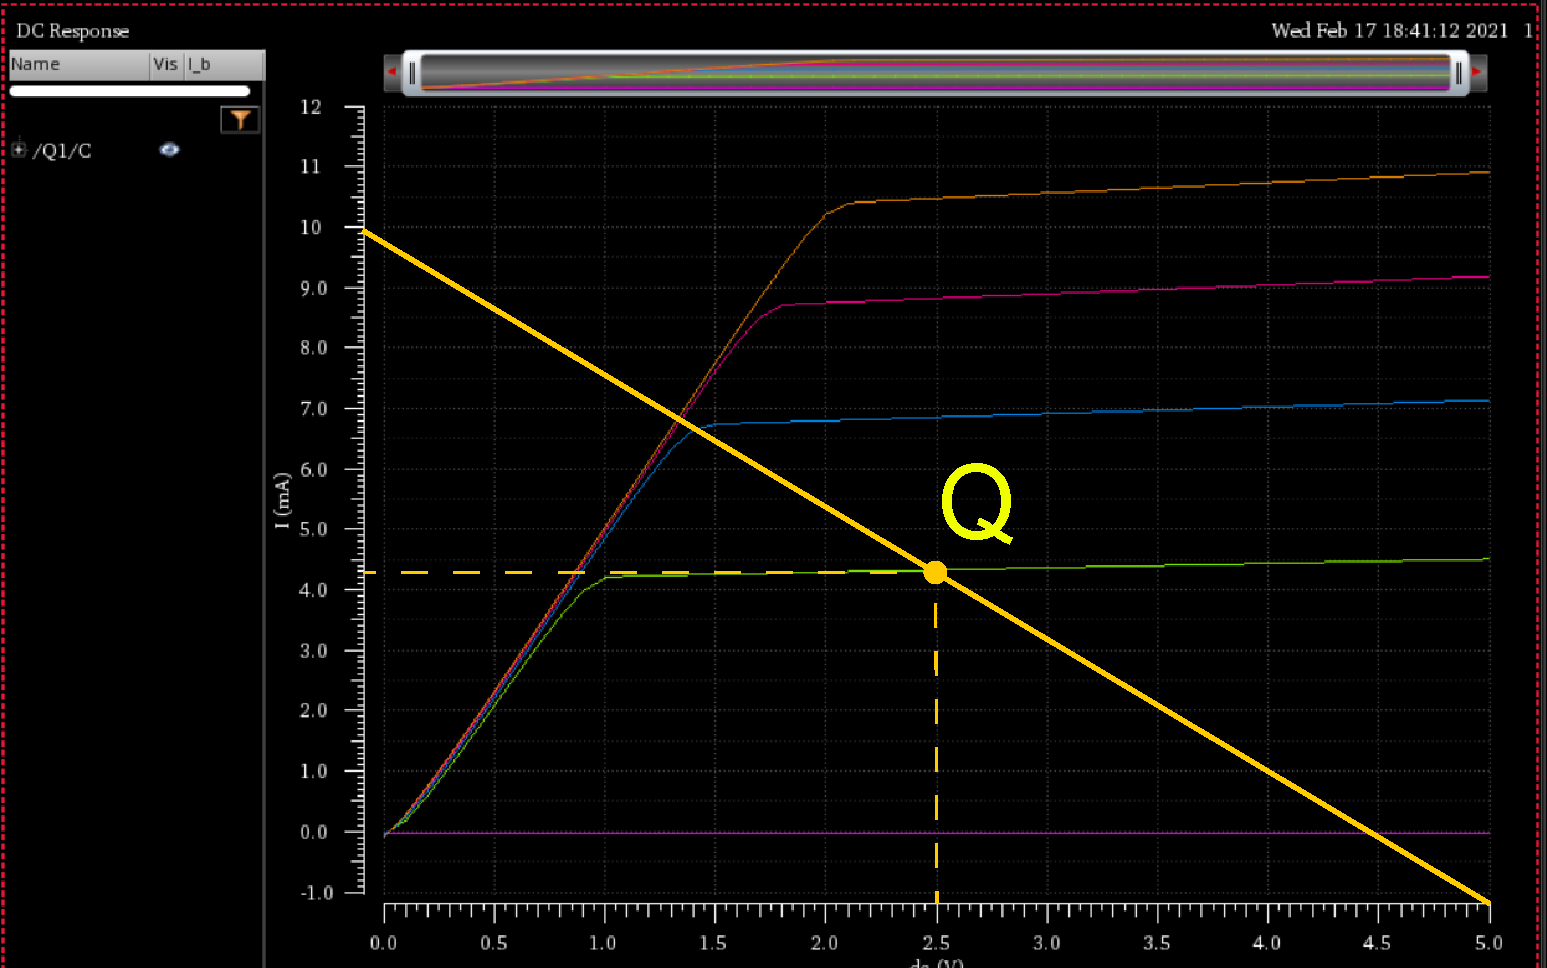
\includegraphics[width=0.45\linewidth]{1.png}}
\caption{Те що выводить моя програма.}
\label{ris1}
\end{figure}



\begin{table}[h]
\begin{center}
\caption{Підсумовуюча таблиця}
\begin{tabular}{|c|c|c|c|c|}
\hline
\multirow{2}{*}{№ сховища} & \multirow{2}{*}{\begin{tabular}[c]{@{}c@{}}Наявність\\ місць\end{tabular}} & \multirow{2}{*}{\begin{tabular}[c]{@{}c@{}}Розміщення\\ Людей\end{tabular}} & \multicolumn{2}{c|}{Додатково установити}                                                                                           \\ \cline{4-5}
                           &                                                                            &                                                                             & \begin{tabular}[c]{@{}c@{}}Кількість і тип\\ ФВК чи ЕРВ\end{tabular} & \begin{tabular}[c]{@{}c@{}}Ємність для\\ води,л\end{tabular} \\ \hline
1                          & 320                                                                        & 330                                                                         & 3 ФВК-2                                                              & 171                                                          \\ \hline
2                          & 156                                                                        & 150                                                                         & 1 ФВК-2                                                              & 54                                                           \\ \hline
\end{tabular}
\end{center}
\end{table}





Висновок: необхідно забезпечити сховища більшою кількістю ємностей з питною водою, а також додати відсутні ФВК.





\end{document}
